% Capítulo 3
\chapter{Arquitetura}

ARASH (Robô Antropomórfico Aumentado com Sentido de Ser Humano), é um robô de 7,5 Kg e 1 metro de altura. Possuindo 20 graus de liberdade (ou DOF, do inglês \textit{degrees of freedom}), ele tenta imitar a configuração humana, tanto em suas juntas quanto em suas proporções. Em suas juntas, ARASH possui motores MX-28, MX-64 e MX-106, dependendo da carga suportada. Existe um computador \textit{mini-box} que serve como controlador principal e uma placa microcontroladora \textit{OpenCM9.04} que serve de interface entre o controlador principal e os motores.

\section{Visão Geral}
\label{sec:architecture:overview}

Com o passar dos antos, a arquitetura distribuída é vem sendo cada vez mais adotada na robótica. A ideia é que cada componente funcione de forma independente para evitar que uma eventual falha derrube todo o sistema. Componentes individuais podem ser adicionados, ou substituídos, a medida em que melhorias, ou novas capacidades, sejam implementadas.

\begin{figure}[htb]
	\centering
	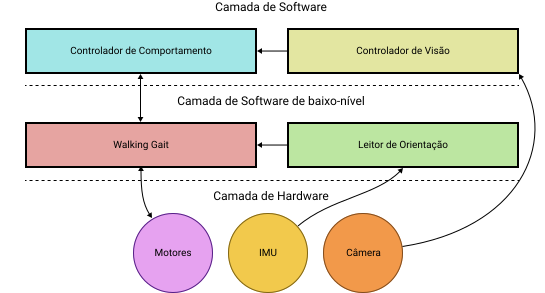
\includegraphics[scale=1]{imagens/svg/softwarearchitecture-flow}
	\caption{Visão simplificada da arquitetura do sistema e seus fluxos.}
	\label{fig:softwarearchitecture:overview}
\end{figure}

Na figura~\ref{fig:softwarearchitecture:overview} é possível observar os principais componentes, e o fluxo de dados entre eles, envolvidos no processo qualquer tarefa básica. Esses componentes podem ser executados em diferentes camadas do sistema. Na arquitetura, existem 3 camadas principais que podem ser descritas independentemente: A camada de software, a de software de baixo nível, e a de hardware.

Na camada de \textit{hardware}, a mais inferior na figura~\ref{fig:softwarearchitecture:overview}, estão a câmera, a IMU e os motores utilizados nas juntas. Os motores serão melhor descritos na subseção sobre atuadores (subseção~\ref{subsec:Architecture:Atuators}). A IMU, \textit{inertial measurement unit}, que é um sensor eletrônico capaz de medir as forças sofridas por um corpo, é utilizada para ler a orientação do corpo do robô.

A camada de software de baixo nível é responsável pelo processamento de dados da \textit{IMU}, juntamente com a execução do \textit{walking gait}. Esta camada roda dentro da placa microcontroladora \textit{Robotis.Co OpenCM9.04} (com um processador \textit{32bit ARM Cortex-M3}, memória \textit{flash} de 128Kb e 20Kb de \textit{SRAM}), \textit{arduino-like}.

A camada de software é executada dentro do ``controlador principal'', que é um computador \textit{mini-box PC MAXData QutePC-3001} com um processador 64 bits de dois núcleos Intel\copyright{} Celeron\copyright{} 847E (1,1GHz e 2MB de \textit{cache}), rodando o Ubuntu 14.04. Esta camada é responsável por rodar os componentes de software e enviar comandos de controle para a camada inferior de baixo nível.

\subsection{Visão}

Visão não é o foco deste trabalho. Entretanto, uma explanação geral é necessária afim de melhor entender o funcionamento geral do sistema.

\begin{figure}[h!]
	\centering
	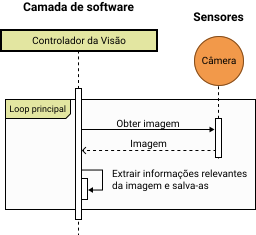
\includegraphics[scale=1]{imagens/svg/softwarearchitecture-vision}
	\caption{Diagrama de sequência do componente de visão.}
	\label{fig:softwarearchitecture:vision}
\end{figure}

O controle de visão é um software que conecta-se via USB com a câmera, analisando as imagens e extraindo informações relevantes à execução da tarefa do robô. De forma geral, podemos abstrair seu funcionamento em duas \textit{threads} distintas:

A primeira é o \textit{loop} principal -- representada na figura \ref{fig:SoftwareArchitecture:Vision} --, onde, sequencialmente, o controlador obtém a imagem da câmera. Em seguida, a extração de informações é realizada. Esse processo depende da tarefa que o robô deve realizar; tais como detectar a bola, os adversários e as linhas do campo, em caso de futebol ou detectar as linhas guia da pista de corrida no caso da maratona. Em seguida, tudo o que foi encontrado é salvo para futuras consultas até que a próxima iteração ocorra e os dados sejam atualizados.

A segunda \textit{thread}, visualizada na figura~\ref{fig:softwarearchitecture:software}, do controle de visão executa o sistema de comunicação que pode ser implementado de várias maneiras, desde objetos \textit{JSON} sendo transmitidos via \textit{UDP} até um \textit{message broker} com filas de consumo. Ao receber a mensagem de solicitação das informações, responde serializando os dados que ficaram salvos na primeira \textit{thread}, fornecendo as informações com atraso mínimo.

\subsection{Controlador de Comportamento}

O controlador de comportamento implementa a tarefa que deve ser realizada pelo robô. Ele funciona como um gerente que coordena outros componentes, recebendo informações e enviando comandos com ações específicas serem executadas. Na figura~\ref{fig:softwarearchitecture:software} é possível observar a sequência de passos realizados pelo controlador de comportamento.

No caso de uma partida de futebol, o controlador de comportamento ``jogador'' consulta o componente de visão, que responde a posição da bola, previamente obtida durante o processo da figura~\ref{fig:softwarearchitecture:vision}. Em seguida, baseado nessas informações o comportamento envia o comando ao \textit{walking gait} para caminhar na direção correta.

\begin{figure}[h!]
	\centering
	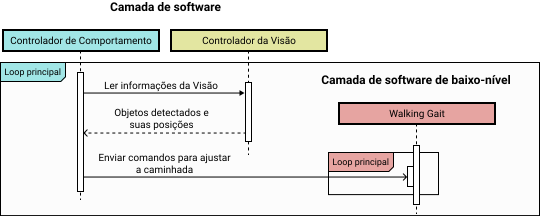
\includegraphics[scale=1]{imagens/svg/softwarearchitecture-software}
	\caption{Diagrama de sequência do controlador de comportamento e suas dependências.}
	\label{fig:softwarearchitecture:software}
\end{figure}

\subsection{\textit{Walking Gait} e Leitor de Orientação}

O componente \textit{walking gait} coordena e executa a caminhada. Ele monitora a USB aguardando os comandos de controle que contém as velocidades da caminhada, enviados a partir do controlador principal.

O componente leitor de orientação desempenha um papel importante dentro do \textit{walking gait}. Ele é o responsável pela verificação da orientação da rotação do torso, uma vez que a \textit{IMU} está situada nas costas de Arash. Desta forma, o \textit{walking gait} faz correções nas juntas para compensar um eventual desvio na trajetória.

\begin{figure}[b!]
	\centering
	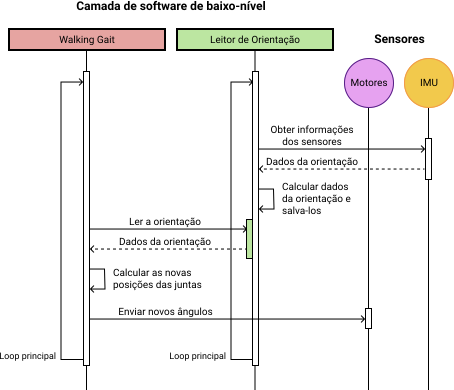
\includegraphics[scale=1]{imagens/svg/softwarearchitecture-lowlevel}
	\caption{Diagrama de sequência do \textit{walking gait} e do leitor de orientação.}
	\label{fig:softwarearchitecture:lowlevel}
\end{figure}

\subsection{Graus de Liberdade e Atuadores}
\label{subsec:architecture:Atuators}

\todo{Adicionar um parágrafo introdutório.}
PARAGRAFO INTRODUTÓRIO.

Tão importante quanto a configuração das juntas é a orientação dos atuadores para que os cálculos funcionem como o esperado.

\begin{figure}[htb]
	\centering
	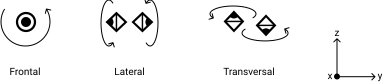
\includegraphics[scale=1]{imagens/svg/actuators-orientation}
	\caption{Orientação dos movimentos dos atuadores}
	\label{fig:ActuatorsOrientation}
\end{figure}

A figura~\ref{fig:ActuatorsOrientation} é possível ver as possíveis orientações dos atuadores. Elas são referenciadas ao longo do trabalho como frontal, lateral e transversal.

Atuadores com orientação frontal -- ou simplesmente, atuadores frontais -- propiciam rotação orientada pelo eixo $X$, que está aponta para o leitor (para fora do papel). Esse tipo de rotação também é referida como \textit{roll}.

Atuadores laterais apontam para direita ou esquerda. Eles apresentam rotação com base no eixo $Y$ (plano $XZ$), também conhecida como rotação \textit{pitch}. Analogamente, atuadores transversais apontam para cima ou baixo, com base no eixo $Z$ (plano $XY$), com movimento de rotação conhecido como \textit{yaw}.

Na figura~\ref{fig:ArashSchematics}, observa-se o esquema de orientação doas atuadores aplicada no diagrama das juntas de Arash. Ainda na mesma figura, os ``triângulos pretos preenchidos'' representam apenas o fim de uma cadeia de atuadores. Assim, estes símbolos representam as mãos, que não possuem atuadores, e a ponta da cabeça, onde encontra-se a câmera. 

Estas orientações são importantes durante os cálculos dos ângulos enviados às juntas. Já que a inconsistência do modelo matemático e o robô causará inversão de movimentos durante a caminhada, causando movimentos estranhos e possíveis danos.

Em Arash, todos os atuadores utilizados são produzidos pela Robotics.Co. Porém, devido a variação de carga nas diversas juntas, foram utilizados diferentes  modelos da série MX. Esta decisão de projeto diminui bastante o custo final do robô.

\begin{figure}[htb]
	\centering
	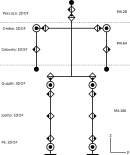
\includegraphics[scale=1]{imagens/svg/arash-schematics}
	\caption{Diagrama de orientação dos atuadores de Arash}
	\label{fig:ArashSchematics}
\end{figure}

No pescoço, onde a carga é bem leve, ``MX-28'' são suficientes. Dois atuadores, um na posição transversal (o atuador mais baixo) que fornece o movimento panorâmico a cabeça e outro na posição horizontal, fornecendo o movimento de inclinação vertical da cabeça.

Nos braços, que podem sofrer uma carga maior, atuadores ``MX-64'' são utilizados. Isso é importante já que existem modalidades de competições, como o levantamento de peso, que testam a capacidade do carregamento de cargas.

Para as pernas, foram utilizados atuadores ``MX-106'' que são mais poderosos que os anteriores. Entretanto, na fase de projeto, simulações mostraram que durante o movimento de levantar-se do chão (em caso da recuperação de uma possível queda), o torque nas juntas do joelho era levado ao máximo suportado pelo ``MX-106'', podendo assim levar este motor à falha. Desta forma, 2 atuadores sincronizados passaram a formar esta junta, afim de proporcionar dividir a força necessária entre dois motores. Esta junta dupla não oferece nenhum impacto na implementação, já que os motores da série ``MX-106'' oferecem a capacidade de serem ligados e sincronizados via \textit{hardware}. Assim, a nível de software controla-se apenas 1 único atuador. Desta forma, apesar das 20 DOF, Arash possui 22 motores.

\section{A nova arquitetura}

De acordo com os problemas já apresentados, esta seção irá apresentar e justificar as mudanças realizadas na arquitetura original apresentada na seção~\ref{sec:architecture:overview}.

\begin{figure}[h!]
	\centering
	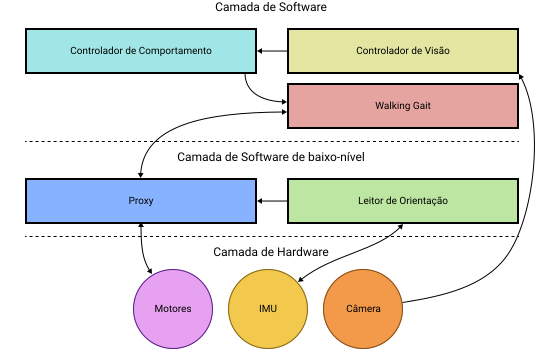
\includegraphics[scale=1]{imagens/svg/softwarearchitecture-newproposal}
	\caption{Diagrama de orientação dos atuadores de Arash}
	\label{fig:softwarearchitecture:newproposal}
\end{figure}

A figura~\ref{fig:softwarearchitecture:newproposal} mostra o \textit{walking gait} em sua nova camada, funcionando dentro do controlador principal, e um novo compontente chamado \textit{proxy} é apresentado como interface entre os motores e o \textit{walking gait}.

O componente \textit{proxy} implementa a comunicação com o controlador principal via USB @ 1Mbps.
